\begin{figure}

\centering

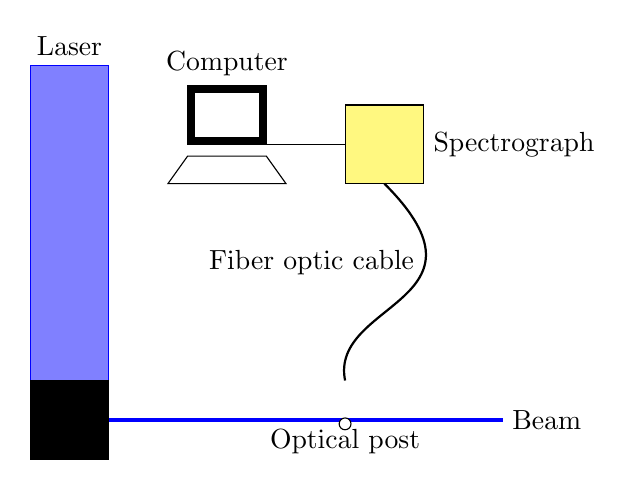
\begin{tikzpicture}

% Laser
\filldraw [fill=blue!50!white, draw=blue] ( 0, 5 ) rectangle ++( 1, -4 );
\filldraw [black] ( 0, 1 ) rectangle ++( 1, -1 );

% Beam
\draw [very thick, blue] ( 1, 0.5 ) -- ++( 5, 0 );

% Optical post
\filldraw [fill=white, draw=black] ( 4, 0.45 ) circle ( 0.075 );
% Computer
\filldraw [black] ( 2, 4 ) rectangle ++( 1, 0.75 );
\filldraw [white]( 2.1, 4.1 ) rectangle ++( 0.8, 0.55 );
\draw ( 2, 3.85 ) -- ++( 1, 0 ) -- ++( 0.25, -0.35 ) -- ++( -1.5, 0 ) -- cycle;

\draw ( 3, 4 ) -- ++( 1, 0 );

% Spectrometer
\filldraw [fill=yellow!50!white, draw=black] ( 4, 3.5 ) rectangle ++( 1, 1 );

% Optical fiber
\draw [thick] ( 4.5, 3.5 ) .. controls +( 1.5, -1.5 ) and +( -0.2, 1 ) .. ++( -0.5, -2.5 );

% Labels
\node at ( 0.5, 5 ) [above] {Laser};
\node at ( 2.5, 4.75 ) [above] {Computer};
\node at ( 5, 4 ) [right] {Spectrograph};
\node at ( 5, 2.5 ) [left] {Fiber optic cable};
\node at ( 4, 0.5 ) [below] {Optical post};
\node at ( 6, 0.5 ) [right] {Beam};

\end{tikzpicture}

\caption[Schematic of the laser calibration experiment]{The figure above shows the schematic of the experiment performed to calibrate the wavelength of the laser output. The laser output (containing mostly UV, but also a small portion of the fundamental frequency) is glanced off a steel optical post. The scattered light is gathered by a fiber optic cable and sent to a spectrometer. The spectrum is analyzed to track the location of the fundamental frequency with tuner position. The UV peak is not tracked as the spectrometer is not calibrated for that wavelength.}

\label{fig:laserCalibration}

\end{figure}

